% Small, maintainable exercise include file.
% Responsibilities are split into includes under `exercises.d/`:
% - `input-path.tex`      : sets `\input@path` for subvariant inputs
% - `setup-counter.tex`   : ensures the `exercise` counter exists
% - `include-exercise.tex`: defines `\IncludeExercise{<path>}` wrapper
% The actual exercise inclusions are then simple calls to \IncludeExercise{<path>}.

% Load path, counter and the include wrapper (keeps this file minimal)
% Ensure TeX looks for subvariant files in the exercise folder when main.tex uses relative \input
\makeatletter
\def\input@path{{../../../ExerciseDatabase/matematica/P4_funcoes/4-funcao_inversa/determinacao_analitica/MAT_P4FUNCOE_4FX_DAX_003/}}
\makeatother

% Define exercise counter if not already defined (defensive)
\makeatletter
\@ifundefined{c@exercise}{\newcounter{exercise}}{}
\makeatother

% Define a simple wrapper command to include an exercise file and
% print a standardized heading. The wrapper toggles the style flag
% `\showexerciciotitle` (defined in style.tex) so the included
% exercise does not duplicate its own heading.
\providecommand{\IncludeExercise}[1]{%
  \begingroup
    \refstepcounter{exercise}%
    \noindent\textbf{Exercício \theexercise.}\par
    \showexerciciotitlefalse
    \input{#1}%
    \showexerciciotitletrue
  \endgroup
}


% Exercício 1, rascunho: (Escolha múltipla) Quais dos seguintes gráficos representa uma função crescente? 

\exercicio{
    Quais dos seguintes gráficos representa uma função crescente?
    \begin{figure}[H]
        \centering
        % Linha superior: Opção A e B
        \begin{minipage}[b]{0.48\textwidth}
            \centering
            \begin{tikzpicture}
                \begin{axis}[
                    axis lines = middle,
                    xlabel = $x$,
                    ylabel = {$f(x)$},
                    ymin=-1, ymax=5,
                    xmin=-1, xmax=5,
                    domain=0:4,
                    samples=100,
                    width=\linewidth,
                    height=4cm,
                ]
                \addplot[blue, thick] {x}; % Opção A: linha crescente
                \end{axis}
            \end{tikzpicture}
            \par\smallskip\textbf{Opção A}
        \end{minipage}\hfill
        \begin{minipage}[b]{0.48\textwidth}
            \centering
            \begin{tikzpicture}
                \begin{axis}[
                    axis lines = middle,
                    xlabel = $x$,
                    ylabel = {$f(x)$},
                    ymin=-1, ymax=5,
                    xmin=-1, xmax=5,
                    domain=0:4,
                    samples=100,
                    width=\linewidth,
                    height=4cm,
                ]
                \addplot[red, thick] {-x + 4}; % Opção B: linha decrescente
                \end{axis}
            \end{tikzpicture}
            \par\smallskip\textbf{Opção B}
        \end{minipage}

        \vspace{6pt}

        % Linha inferior: Opção C e D
        \begin{minipage}[b]{0.48\textwidth}
            \centering
            \begin{tikzpicture}
                \begin{axis}[
                    axis lines = middle,
                    xlabel = $x$,
                    ylabel = {$f(x)$},
                    ymin=-1, ymax=5,
                    xmin=-1, xmax=5,
                    domain=0:4,
                    samples=100,
                    width=\linewidth,
                    height=4cm,
                ]
                \addplot[green, thick] {2}; % Opção C: linha constante
                \end{axis}
            \end{tikzpicture}
            \par\smallskip\textbf{Opção C}
        \end{minipage}\hfill
        \begin{minipage}[b]{0.48\textwidth}
            \centering
            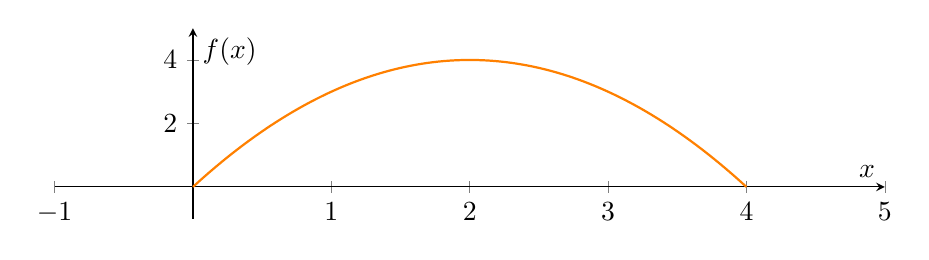
\begin{tikzpicture}
                \begin{axis}[
                    axis lines = middle,
                    xlabel = $x$,
                    ylabel = {$f(x)$},
                    ymin=-1, ymax=5,
                    xmin=-1, xmax=5,
                    domain=0:4,
                    samples=100,
                    width=\linewidth,
                    height=4cm,
                ]
                \addplot[orange, thick] {4 - (x-2)^2}; % Opção D: curva não crescente em geral
                \end{axis}
            \end{tikzpicture}
            \par\smallskip\textbf{Opção D}
        \end{minipage}
    \end{figure}
}

% Exercício 2, rascunho: (Escolha múltipla) Quais dos seguintes gráficos representa uma função descrescente? (Comprar curvas exponenciais, logaritmos e parabolas)

\exercicio{
    Quais dos seguintes gráficos representa uma função descrescente?
    \begin{figure}[H]
        \centering
        % Linha superior: Opção A e B
        \begin{minipage}[b]{0.48\textwidth}
            \centering
            \begin{tikzpicture}
                \begin{axis}[
                    axis lines = middle,
                    xlabel = $x$,
                    ylabel = {$f(x)$},
                    ymin=-1, ymax=5,
                    xmin=-1, xmax=5,
                    domain=0:4,
                    samples=100,
                    width=\linewidth,
                    height=4cm,
                ]
                \addplot[blue, thick] {exp(0.3*x)}; % Opção A: curva exponencial (e^{0.3x})
                \end{axis}
            \end{tikzpicture}
            \par\smallskip\textbf{Opção A}
        \end{minipage}\hfill
        \begin{minipage}[b]{0.48\textwidth}
            \centering
            \begin{tikzpicture}
                \begin{axis}[
                    axis lines = middle,
                    xlabel = $x$,
                    ylabel = {$f(x)$},
                    ymin=-1, ymax=5,
                    xmin=-1, xmax=5,
                    domain=0:4,
                    samples=100,
                    width=\linewidth,
                    height=4cm,
                ]
                \addplot[red, thick] {ln(x+1)}; % Opção B: curva logarítmica (ln(x+1))
                \end{axis}
            \end{tikzpicture}
            \par\smallskip\textbf{Opção B}
        \end{minipage}

        \vspace{6pt}

        % Linha inferior: Opção C e D
        \begin{minipage}[b]{0.48\textwidth}
            \centering
            \begin{tikzpicture}
                \begin{axis}[
                    axis lines = middle,
                    xlabel = $x$,
                    ylabel = {$f(x)$},
                    ymin=-1, ymax=5,
                    xmin=-1, xmax=5,
                    domain=0:4,
                    samples=100,
                    width=\linewidth,
                    height=4cm,
                ]
                \addplot[green, thick] {((x-2)^2)/2}; % Opção C: parábola ( (x-2)^2 / 2 )
                \end{axis}
            \end{tikzpicture}
            \par\smallskip\textbf{Opção C}
        \end{minipage}\hfill
        \begin{minipage}[b]{0.48\textwidth}
            \centering
            \begin{tikzpicture}
                \begin{axis}[
                    axis lines = middle,
                    xlabel = $x$,
                    ylabel = {$f(x)$},
                    ymin=-1, ymax=5,
                    xmin=-1, xmax=5,
                    domain=0:4,
                    samples=100,
                    width=\linewidth,
                    height=4cm,
                ]
                \addplot[orange, thick, samples=200] {1/(x+0.5) + 1.5}; % Opção D: hipérbole deslocada
                \end{axis}
            \end{tikzpicture}
            \par\smallskip\textbf{Opção D}
        \end{minipage}
    \end{figure}
}

% Exercício 3, racunho: Completa a seguinte frase: "Uma função é dita constante quando..."

\exercicio{
    Completa a seguinte frase: "Uma função é dita constante quando..."
    \vspace{2cm}    
}

% Exercício 4, rascunho: é apresentado um gráfico de uma função simples (linear/retas e constantes) definida por ramos. 

\exercicio{
    
    O gráfico seguinte representa uma função definida por ramos. Estuda a monotonia da função e calcula os valores de \(\Delta x\), \(\Delta y\) e \(\frac{\Delta y}{\Delta x}\).
    
    \begin{figure}[H]
        \centering
        \begin{tikzpicture}
            \begin{axis}[
                axis lines = middle,
                xlabel = $x$,
                ylabel = {$f(x)$},
                ymin=-1, ymax=5,
                xmin=-1, xmax=5,
                domain=0:4,
                samples=100,
                width=0.7\linewidth,
                height=6cm,
            ]
            % Definir a função por ramos
            % Ramos com domínios explícitos
            \addplot[blue, thick, domain=0:2, samples=50] {x};        % Ramo 1: y = x para 0 ≤ x < 2
            \addplot[blue, thick, domain=2:3, samples=2] {2};         % Ramo 2: y = 2 para 2 ≤ x < 3
            \addplot[blue, thick, domain=3:4, samples=50] {5 - x};    % Ramo 3: y = 5 - x para 3 ≤ x ≤ 4
            % Marcadores nos extremos incluídos (0,0), (2,2), (3,2), (4,1)
            \addplot[only marks, mark=*, mark options={fill=blue}, mark size=2pt] coordinates {(0,0) (2,2) (3,2) (4,1)};
            \end{axis}
        \end{tikzpicture}
    \end{figure}

\vspace{7cm}
}
% Exercicio 5, rascunho: Atenta na função f(x) = x^2, estuda o \frac{\triang y}{\triang x} do intervalo [0, 4].
\exercicio{
    Atenta na função \(f(x) = x^2\), estuda o \(\frac{\Delta y}{\Delta x}\) do intervalo \([-4, -1]\) e \([0, 4]\).
    
    \vspace{7cm}
}